\documentclass[../Main.tex]{subfiles}

\begin{document}
    

\subsection{Neural Network} \label{network}
    In this chapter we describe the neural network used for style transfer. 
    First we describe it's architecture and specific layers. Then we detail
    pruning procedure used to obtain the final model.
    \subsubsection{Overall network architecture} 
    We follow architecture described in \cite{Li2018}, changing it's components' details 
    in order to enable real time inference. The network consists of two 
    main components - encoder-decoder module and
    transformation module pictured in Figure \ref{fig:overall_network}.
    To perform style transfer encoder is fed with content image
    and style image, producing feature maps cF and sF respectively.
    Next, transformation module transfers sF's statistics onto cF. Resulting 
    feature map is passed through decoder, which creates final image. 
    Thanks to this modular architecture, each style image needs to be encoded
    only once. For both encoder-decoder and
    transformation module we use pretrained models publicly available at 
    \url{https://github.com/sunshineatnoon/LinearStyleTransfer}
    as starting point for further development. Because of implementation details
    of pruning framework we use (each layer can only be used once during 
    feed-forward phase), encoder couldn't be used to encode both content and
    style image. As a consequence we had to include not one, but two copies of encoder
    in our model - one for content images and one for style images. They start of
    with entirely identical set of weights, but progressively diverge from each 
    other during pruning procedure
    
    \begin{figure}[h!]
        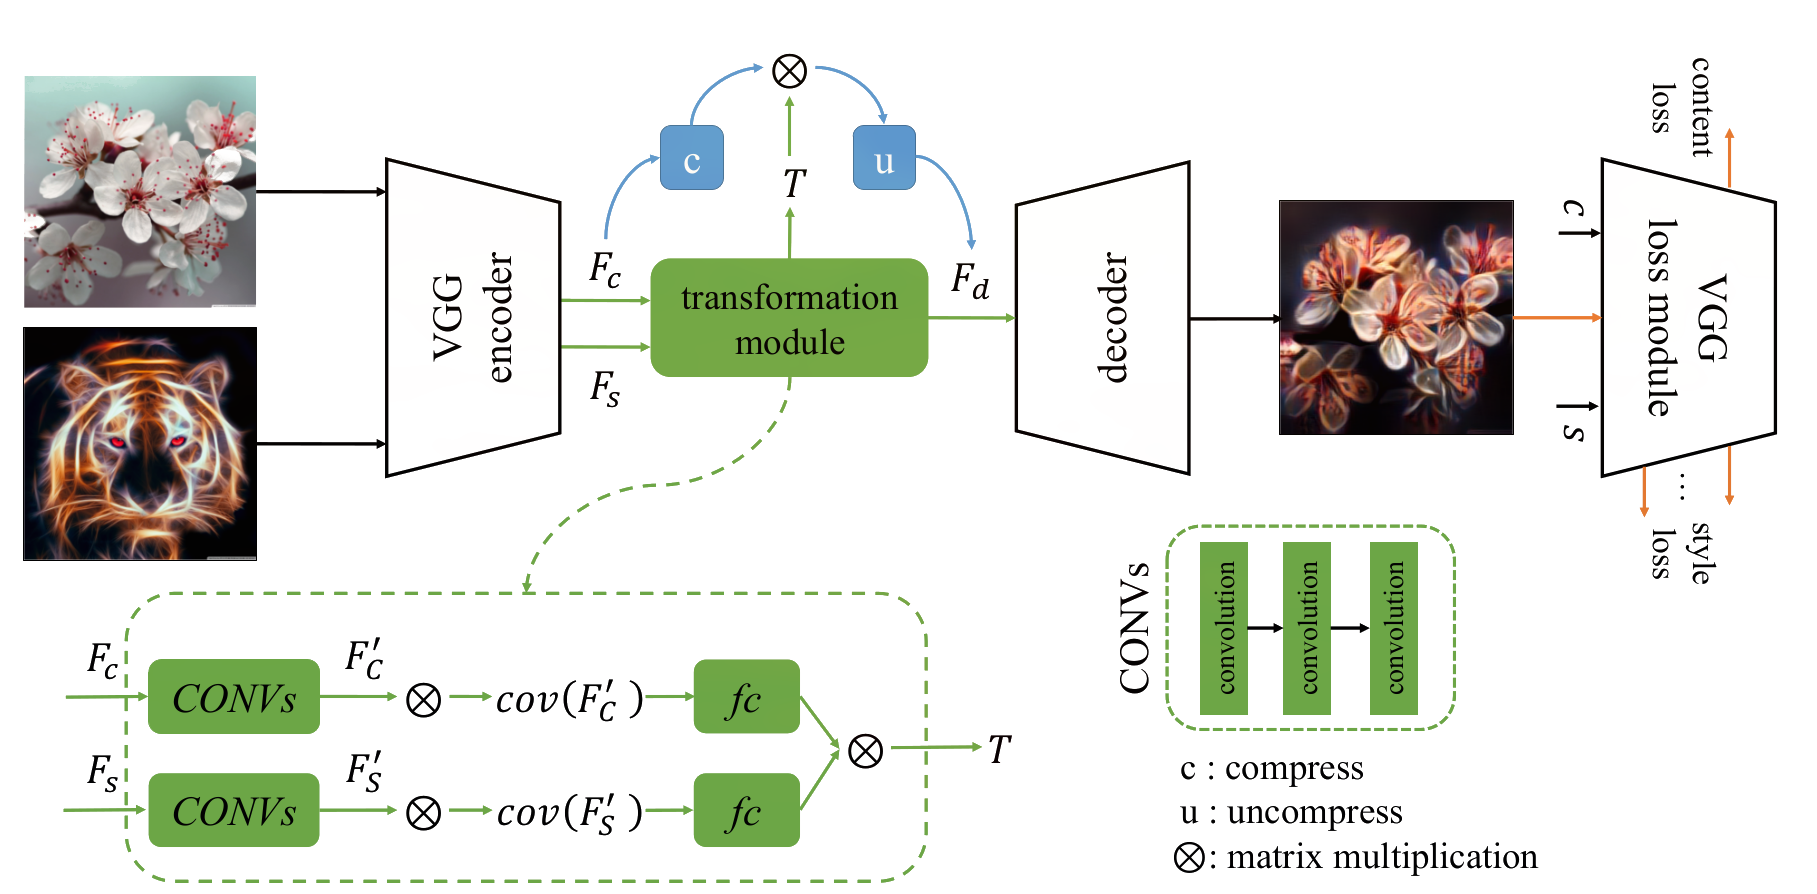
\includegraphics[scale=0.25]{overall_network.png}
        \caption{Overview of the network architecture}
        \label{fig:overall_network}
    \end{figure}
    
    
    \subsubsection{Encoder-decoder}
    Both encoders and decoder are based on first layers of VGG-like \cite{vgg}
    network. VGG is a family of fully convolutional neural networks developed 
    specifically for computer vision task. Full VGG network consists of
    stacked Conv layers with ReLU activation function, interleaved with pooling
    layers performing downsampling, ending with couple of fully
    connected layers and Softmax layer. Such architecture allows for image classification.
    To adapt it for other computer vision tasks like segmentation, object detection,
    tracking, domain adaptation or style transfer, the non-convolutional part
    of network needs to be removed. Depending on task's complexity, desired
    latency and available hardware, vgg-like networks of varying depth can be 
    constructed by simply removing consequent top layers of the network.
    The architecture used by \cite{Li2018} and our pruned version are 
    outlined in table \ref{table:vgg}. 
    
    \begin{table}
    \begin{center}
        \begin{tabular}{|c|c|}
        \hline
         \cite{Li2018} & Our \\
        \hline
          \multicolumn{2}{|c|}{Pointwise Conv(3, 3)} \\
          \hline
          CReLU(3, 64)  & CReLU(3, 16)  \\
          \hline
          CReLU(64, 64) & CReLU(16, 16)  \\
          \hline
          \multicolumn{2}{|c|}{Max Pool x2}      \\
          \hline
          CReLU(64, 128)  & CReLU(16, 32) \\
          \hline
          CReLU(128, 128)  & CReLU(32, 32)\\
          \hline
          \multicolumn{2}{|c|}{Max Pool x2}    \\
          \hline
          CReLU(128, 256) & CReLU(32, 64)\\
          \hline
          CReLU(256, 128) & CReLU(64, 32)\\
          \hline
          \multicolumn{2}{|c|}{Upsample Nearest x2}\\
          \hline
          CReLU(128, 128) & CReLU(32, 32)\\
          \hline
          CReLU(128, 64) & CReLU(32, 16)\\
          \hline
          \multicolumn{2}{|c|}{Upsample Nearest x2}\\
          \hline
          CReLU(64, 64) & CReLU(16, 16) \\
          \hline
          CReLU(64,3) & CReLU(16, 3)\\
          \hline
        \end{tabular}
            \end{center}
        \caption{Encoder-decoder architecture before and after filter pruning.
        The first Conv layer is pointwise convolution with 1x1 kernel, 
        unitary stride, without padding. It has 3 input and 3 output channels.
        \textit{CReLU(a,b)} is Conv layer with \textit{a} input channels and 
        \textit{b} output channels followed by ReLU activation. All of 
        \textit{CReLU}s have 3x3 kernels, unitary stride and and single pixel
        of padding on each of 4 sides. Downsampling and upsampling
        is done with 2x2 kernels and stride 2.
        }
        \label{table:vgg}
    \end{table}
    
    They differ in three aspects:
    \begin{itemize}
        \item \textbf{Padding} - \cite{Li2018} use reflection padding. In many
        models used for style transfer, use of zero padding degrades network's
        performance around the input's edges \cite{johnson2016perceptual}, exhibiting as
        vanishing of style or artifacts (see figure \ref{fig:edges}).
        In such situation adding reflection padding fixes the issue. We replace
        reflection padding with zero padding, because the former one is not 
        implemented within TensorRT used for additional inference speedup
        (see \ref{trt_chapter}). Fortunately described problem is not nearly as visible
        in our model.
        \begin{figure}[h!]
            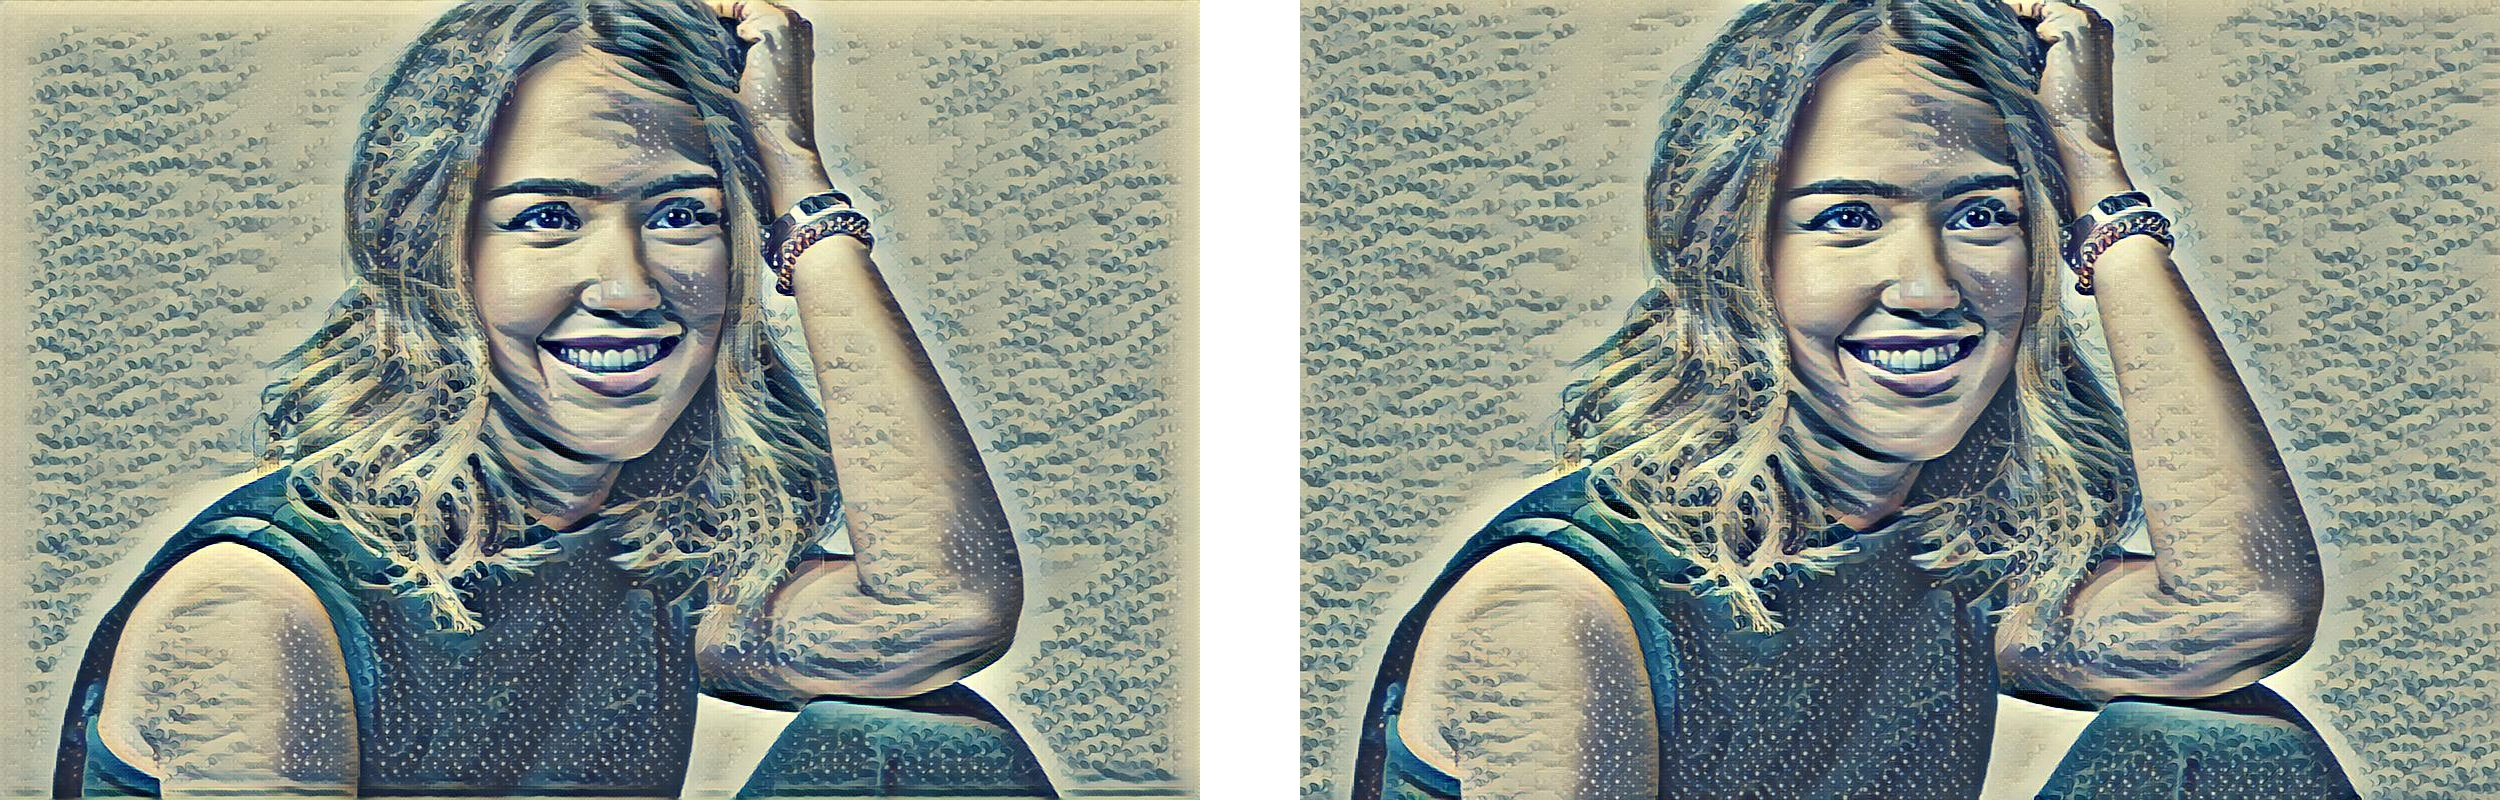
\includegraphics[scale=0.17]{edges.jpg}
            \caption{Result of zero padding (left) and reflection padding (right)
                in \cite{johnson2016perceptual}. Style visibly diminishes around
                the edges in the left image.
            }
            \label{fig:edges}
        \end{figure}
        \item \textbf{Width} of Conv layers. In order to reduce inference time,
        we prune encoder, decoder and part of transformation module
        to only contain $25\%$ of feature maps from the original architecture.
        This provides 
        fivefold speedup on NVIDIA GTX 960 GPU the inference server is ran on 
        (see \ref{speedup} for details).
        \item As described earlier our network consists of two encoders, specialized
        for content and style images respectively. In section \ref{two_encoders}
        we conduct experiments to observe effects of using style encoder for 
        content images and vice-versa.
        
    \end{itemize}


    \subsubsection{Transformation module}
    Transformation module is the component where style is actually transfered
    by matching feature maps' statistics. \cite{huang2017adain} introduced
    statistics matching as style transfer method in form of Adaptive Instance
    Normalization (AdaIN). Their model also consists of encoder, transformation
    module and decoder. Transformation module performs AdaIn on feature maps
    produced by encoder by explicitly matching their means and standard deviations:
    \[ AdaIN(F_C, F_S) = \sigma(F_S)\left( \frac{F_C - \mu(F_C)}{\sigma(F_C)}\right)+\mu(F_S) \]
    where $F_C$ is $n$th content feature map and $F_S$ is $n$th style feature map.
    Transformed feature maps are then decoded to final image. This simple transformation 
    module performs reasonably well for smooth styles (e.g. impressionist paintings),
    but often fails if content or style image contains some sharp edges 
    (e.g. cubist paintings). \cite{Li2018} observe
    AdaIN is in fact an affine transformation of feature map vector $F_C$. 
    This suggests it can be generalized to higher dimensional transformation 
    using matrix multiplication and bias vector. It's then assumed style transfer
    can be performed by an affine transformation conditioned on parameters 
    of style and content image. Using not only mean and variance, but also 
    covariances between individual feature maps enables transferring 
    more sophisticated features. Exact architecture of
    transformation module proposed by \cite{Li2018} is depicted in Figure
    \ref{fig:transform_module}. 
    
        \begin{figure}[h!]
        \centering
            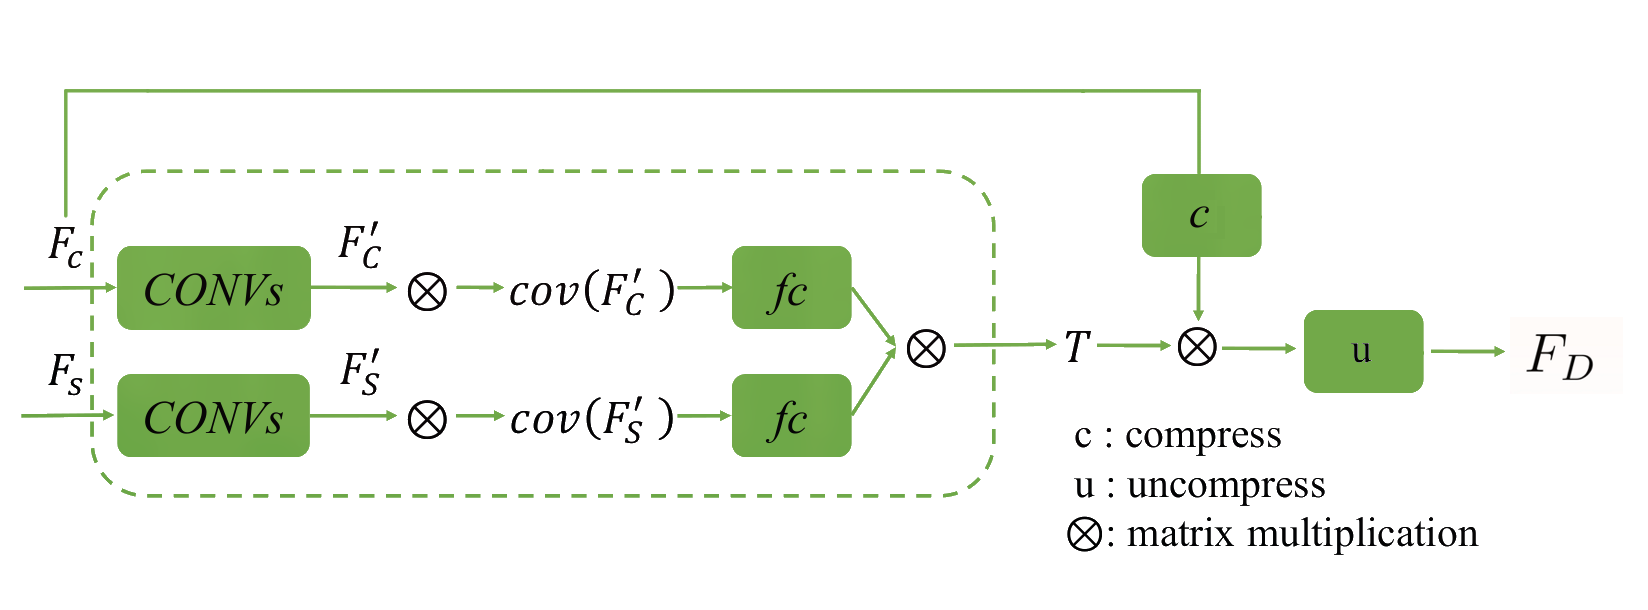
\includegraphics[scale=0.25]{transform_module.png}
            \caption{Architecture of transformation module. $F_C$, $F_S$ and $F_D$
            are content, style and transformed image feature maps respectively.
            $f_c$ is fully connected layer and $T$ is transformation matrix. 
            The submodule in dashed green region is supposed to compute 
            transformation matrix conditioned on style and content images.
            }
            \label{fig:transform_module}
        \end{figure}
        
    First both $F_C$ and $F_S$ are centered around 0 channelwise, that is their respective 
    means for each channel are subtracted. They are then passed through short series of separate 
    convolutional layers with ReLU non-linearity. It's important they are separate,
    since we care about different features in content and style image. Then they 
    are matrix-multiplied with their respective transposes which results in
    their uncentered covariance matrices. Each of these matrices is then fed 
    through fully connected layer, which is supposed to select which covariances
    are the most important. Results of fc layers are then matrix-multiplied
    with each other, which gives us the final style transformation matrix $T$.
    On parallel path $F_C$ vector is compressed to the size of $T$. Compressed 
    $F_C$ is matrix-multiplied with $T$ (this the moment style is transferred)
    and uncompressed to the original size of $F_C$. Lastly mean vector of original $F_S$
    is added. This way means of $F_D$'s channels and $F_S$'s channels are alligned
    exactly.
    
    
    
    
    
    
    
    

\subsection{Pruning}
    In this chapter we describe the pruning algorithm and the pruning procedure 
    used to obtain final network.
    \subsubsection{Filter pruning} 
    Filter pruning is a type of structured pruning in which the smallest unit considered by
    algorithm is convolutional filter. Convolutional layer transforms feature maps
    $x_i \in \mathbb{R}^{n_i \times h_i\times w_i}$ into
    feature maps  $x_{i+1} \in \mathbb{R}^{n_{i+1}h_{i+1} \times w_{i+1}}$ by applying
    $n_{i+1}$ 3D $n_i \times k \times k$ filters $F_{i,j}$. Based on some criterion, filter pruning 
    algorithm removes selected filters to reduce required storage and inference time.
    If filter $F_{i,j}$ is pruned, then so is $j$th feature map of $i$th layer. 
    Filters of the next layer which were convoluted with this feature map are no longer needed 
    and can also be removed. 
    The criterion by which our algorithm selects filters is  
    $\ell_1$ norm, that is $\sum_{i,j}|f_{i,j}|$ where summation is done
    over all filter's values, suggested by \cite{li2016pruning}.
    Intuition behind this and similar criteria (e.g. using 
    $\ell_p$ norm) is that the smaller filter's norm, the smaller it's influence 
    on overall network output. Despite it's simplicity this criterion performs well in practice
    and was adopted by many recent publications \cite{lottery1, lottery2}.
    
    Our algorithm takes as inputs layers which should be pruned and sparsity levels
    respective layers should be pruned to. Pruning changes the network and it's activations' distribution
    very suddenly, so after every removal of filters, network has to be retrained to 
    at least partially regain it's original quality. Pruning can be done at once 
    (so called one shot pruning), 
    where desired sparsity level is achieved just after one epoch or can be 
    spread across multiple epochs.  Retraining is easier in latter scenario,
    as network isn't altered suddenly so significantly. Specifically we use AGP (Automated
    Gradual Pruner) sparsity schedule proposed by \cite{zhu2017prune}. It prunes
    filters rapidly at the beginning, when redundant weights are abundant
    and slows down gradually. \% of filters remaining (called density) after epoch 
    k is given by
    \[ D_k = f_f + (1-f_f)*(1-\tfrac{k}{K})^3 \]
    where $f_f$ is final density and $K$ is total number of epochs
    pruning is performed for. In our case $f_f=0.25$ and $K=10$. Exact densities
    in our schedule our shown in Figure \ref{fig:AGP}. 
    
        \begin{figure}[h!]
            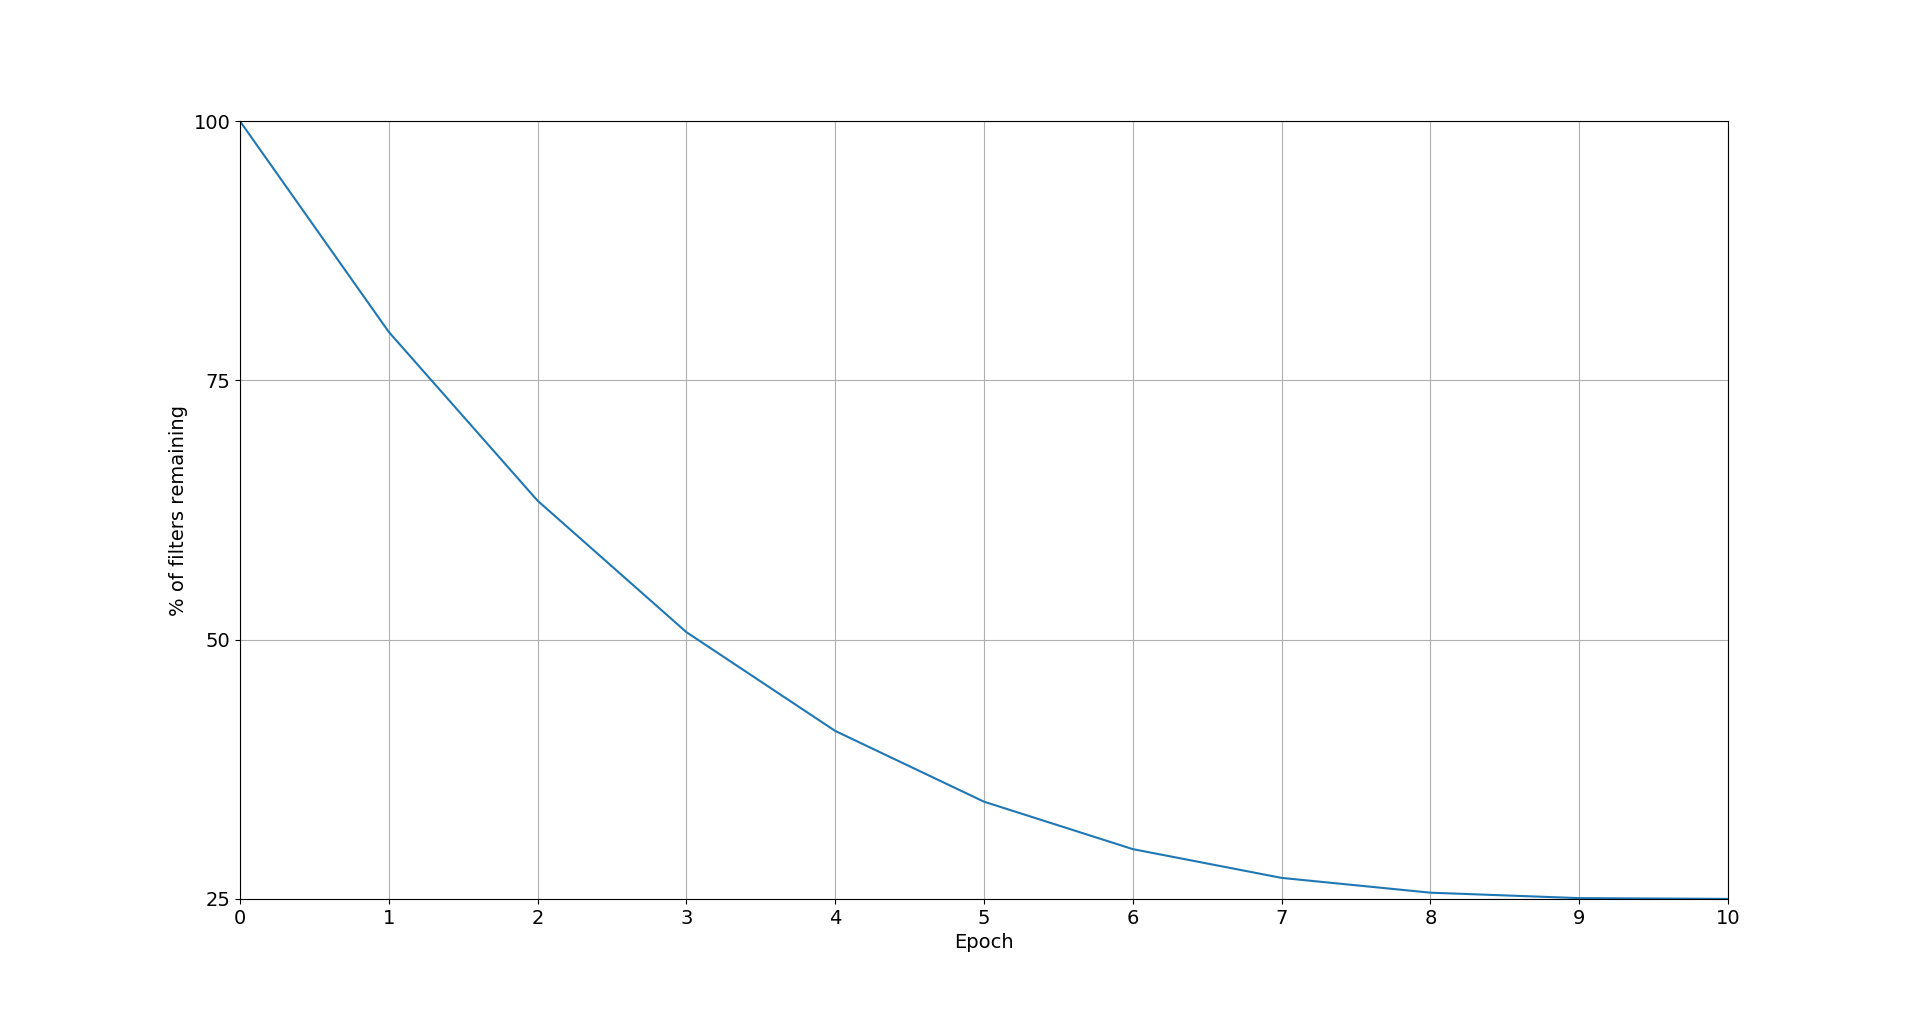
\includegraphics[scale=0.35]{AGP.png}
            \caption{Density of pruned layers after each epoch. 
            }
            \label{fig:AGP}
        \end{figure}
        

    
    \subsubsection{Loss function}
    As can be seen in Figure \ref{fig:overall_network}, losses are computed by
    special VGG19 loss module. The network was pretrained on large dataset for classification
    task and is able to extract useful features for any image. 
    VGG19 is a deep network and it's consecutive
    layers encode different characteristics of image, for example first layers might
    encode colors and texture, while latter layers more abstract features like shapes.
    To compute losses transformed image, content image and
    style image are passed through loss module, which encodes them into $F_{t,i}$, $F_{c,i}$ and 
    $F_{s,i}$ feature maps respectively, where $F_{x,n}$ is feature map computed by $n$th
    ReLU activation layer. \cite{Li2018} find computing style loss combining many $F_{s,i}$
    feature maps yields the best visual effects - they pick $i=2,4,6,10$. For 
    content loss one feature map is enough - $i=10$. Content loss is then computed as 
    MSE between $F_{c,10}$ and $F_{t,10}$. Style loss is given by 
    \[ \sum{MSE(mean(F_{t,i}), mean(F_{s,i})) + MSE(F_{t,i}F_{t,i}^T, F_{s,i}F_{s,i}^T}) \]
    where summation is done over selected layers and MSE is mean squared error.
    $AA^T$ is called Gram matrix of matrix $A$. It serves as $A$'s uncentered covariance.
    Style loss' purpose is then matching statistics of
    style images' distribution and transformed images' distribution.
    Total loss is weighted sum of content loss and style loss:
    \[L=L_{content} + \lambda L_{style}\] \cite{Li2018} use $\lambda=0.02$ and we 
    also find it results in the most appealing visual effects. During pruning and 
    fine-tuning we SGD optimizer to apply gradients. We set learning rate to $10^{-4}$
    and momentum to $0.9$. We use SGD mainly because other optimizers aren't implemented 
    in pruning framework we use. However we also find adaptive optimizers result 
    in instable training of transformation module and gradient explosion.
    
    \subsubsection{Pruning schedule, datasets} 
    Following \cite{Li2018} we MS-COCO \cite{mscoco} as content dataset and Wikiart \cite{wikiart}
    as style dataset. Both of these datasets contain roughly 80000 images. We divide them 
    into 73000 training images and 7000 validation images. Implementing pruning on your own
    requires deep knowledge of used deep learning framework. Luckily there are model 
    minimization libraries for both PyTorch and Tensorflow. While Tensorflow has 
    a builtin library aiding pruning and quantization, PyTorch doesn't have one yet - 
    quantization is in experimental phase and pruning is not available at all. The only 
    software for pruning PyTorch models we are aware of is Distiller \cite{distiller}.
    It's an open source library which implements many structured and unstructured
    pruning algorithms, enables testing quality of quantized models and performing
    knowledge distillation. It's still far from perfect (current version is 0.4.1), but 
    thanks to the open source code, it's easily extendable. Described above
    $\ell_1$ AGP filter pruning is already implemented in Distiller. After specifying
    our network's architecture and datasets, and fixing couple minor bugs 
    we used it to prune and then fine-tune the 
    original model shared by \cite{Li2018} available at
    \url{https://github.com/sunshineatnoon/LinearStyleTransfer}. 
    Pruning phase takes 10 epochs. At the beginning of each epoch scheduled part of filters
    with the lowest $\ell_1$ norm is masked with zeros and frozen for the rest of procedure
    (computation and application of gradients for them is turned off). For the rest of 
    epoch usual training is performed - both content and style datasets are shuffled,
    and network is optimized with consequent mini-batches. During this training,
    network should at least partially recover from performance drop caused by sudden
    change of weights. After 10 epochs, specified
    for each layer level of sparsity is achieved and frozen weights are entirely removed
    from the model - at this moment architecture of the network is altered and physical
    storage required to save the model is reduced. Then comes the fine-tuning phase - 
    network is trained for another
    10 epochs, which should be enough for model to converge to some satisfying state.
    
    Throughout both phases validation loss is measured after each training epoch.
    As final model we pick the one with the lowest validation loss during fine-tuning, 
    which happens to be the one after epoch 18. Training and validation losses are 
    pictured in Figure \ref{fig:wykresy}. Because image reconstruction is fairly 
    easy, content losses remain almost constant during whole process. We see style 
    loss is much more heavily influenced by pruning. Right at the start, mean style loss 
    on training set is right below 2.5, while mean validation loss is over 11. This means 
    model is able to quickly recover and fit to the data even after very aggresive pruning 
    (in AGP scheme first epoch removes the most filters), but regaining generalization requires more
    time. While training style loss drops almost uniformly starting from the 5th epoch, 
    when pruning becomes lighter, the validation set style loss only stabilizes after 10th epoch - 
    when pruning ends. It's important to note that even though validation style loss 
    doesn't change much after 11th epoch, model is still learning and after 18th
    epoch network performs much better than after 11th. This is because the style loss 
    computed by loss module is only a proxy for style difference, which doesn't have 
    any clear mathematical definition. In result value of style loss only partially reflects
    difference in style between two pictures. 
    
    \begin{center}
     \begin{figure}[h!]
            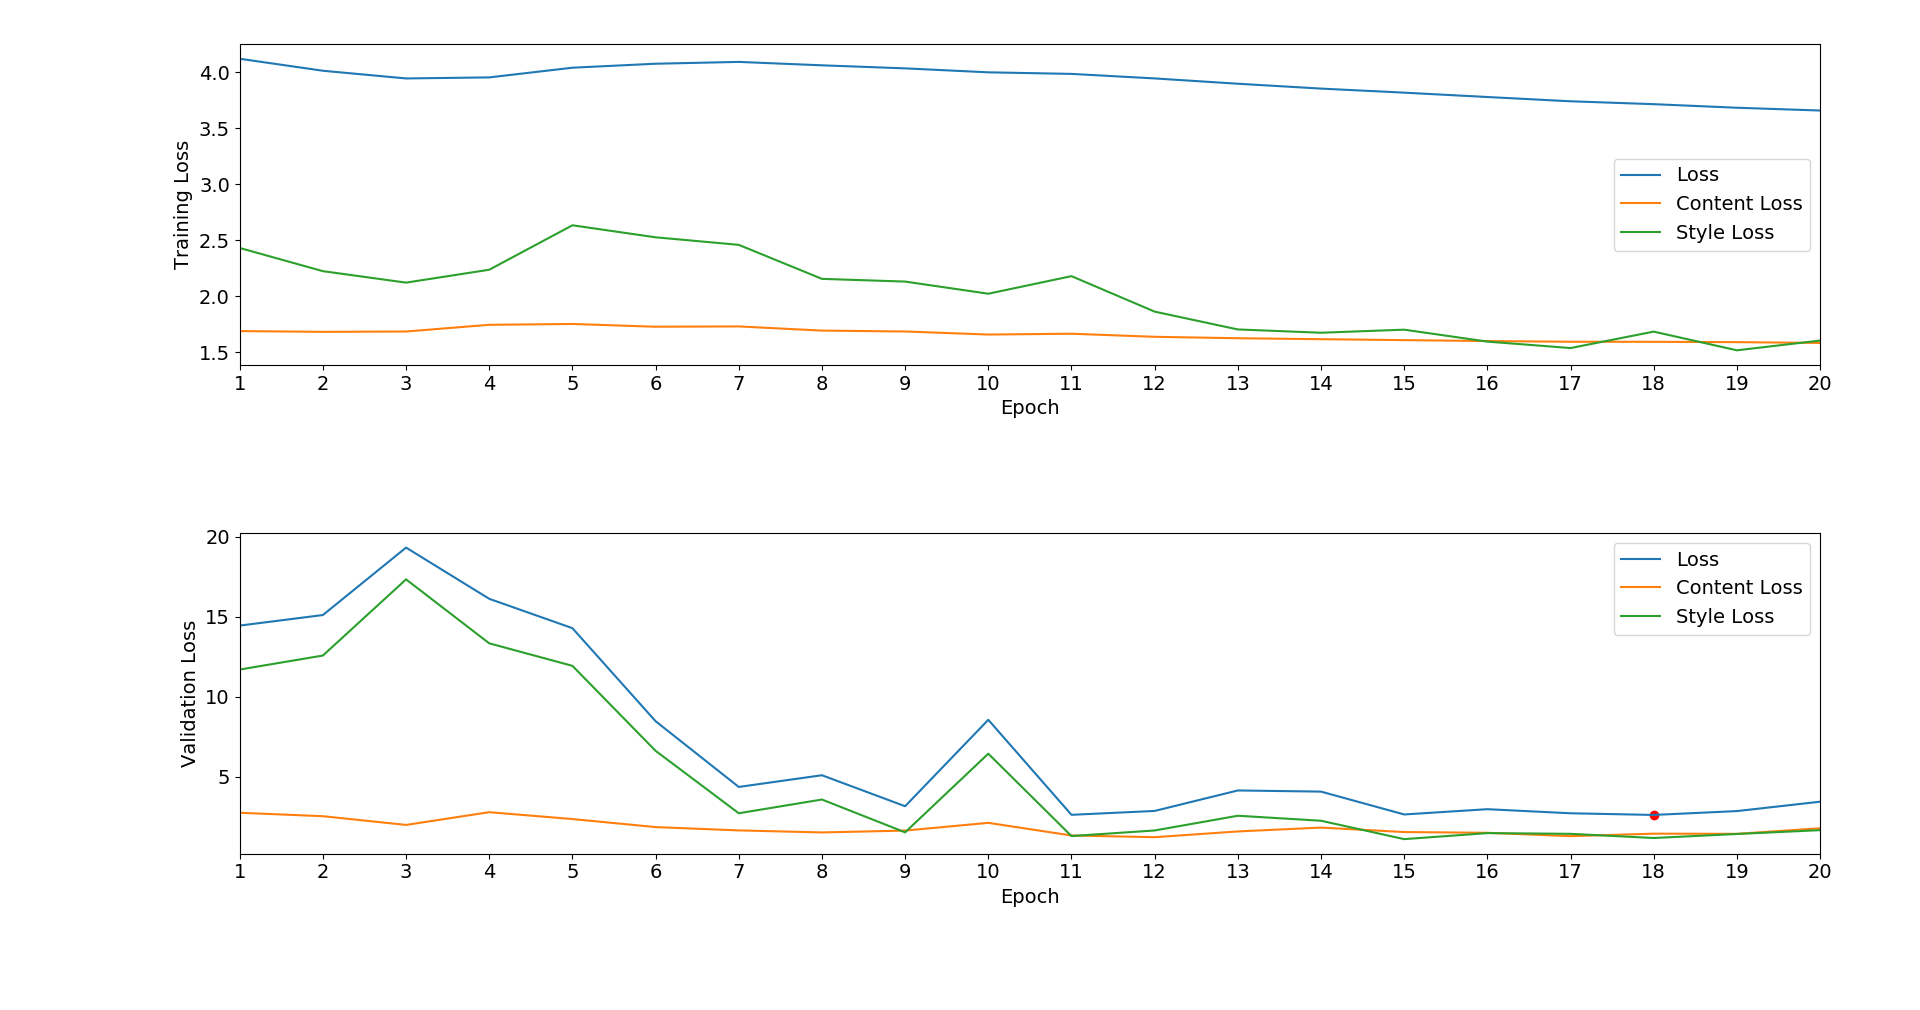
\includegraphics[scale=0.3]{wykresy.png}
            \caption{Mean training and validation losses throughout pruning and fine-tuning
            procedure. Optimal model with minimal validation loss in fine-tuning phase 
            is marked with red dot.
            }
        \label{fig:wykresy}
    \end{figure}
    \end{center}
    




\biblio % Needed for referencing to working when compiling individual subfiles - Do not remove
\end{document}
